\begin{figure*}[t]
\centering
% === LEFT SIDE ===
\begin{minipage}{0.47\textwidth}
    \centering
    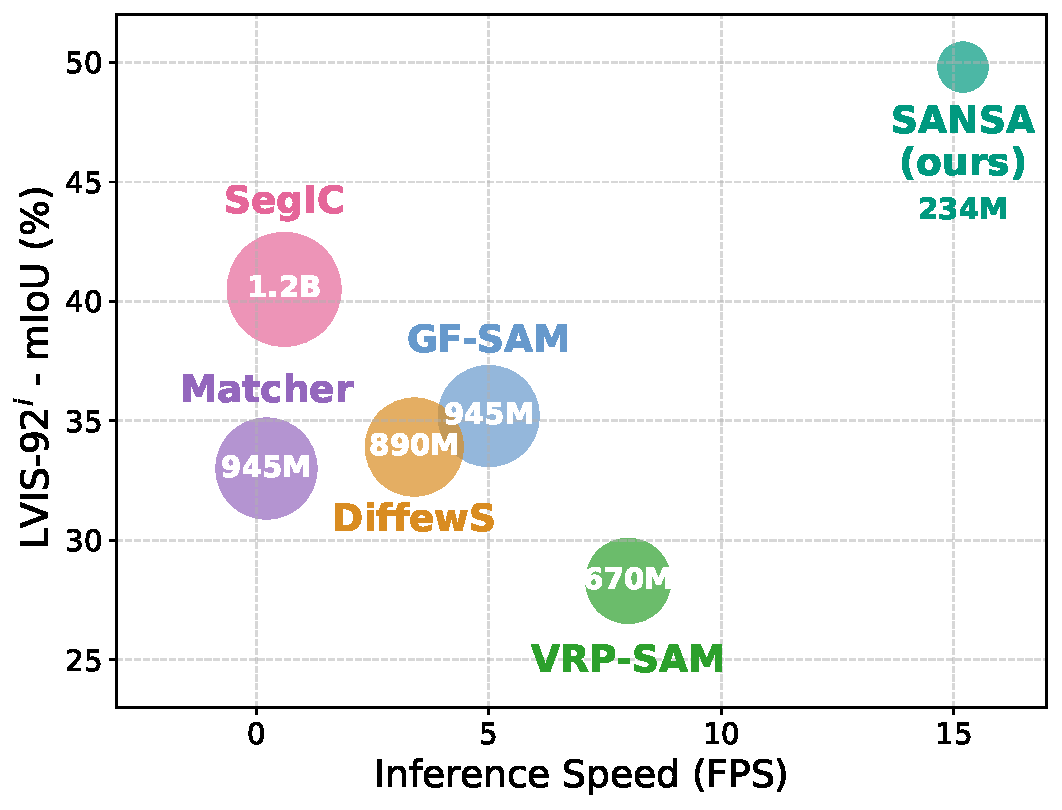
\includegraphics[width=\textwidth]{images/miou_vs_fps.pdf}
    \vspace{-15pt}
    \captionof{figure}{\textbf{Comparison of inference speed and mIoU}, with bubble size representing \#parameters. The plot highlights our superior trade-off.}
    \label{fig:fps_new}
\end{minipage}
\hspace{8pt}
% === RIGHT SIDE  ===
\begin{minipage}{0.49\textwidth}
    
    \setlength\tabcolsep{2.5pt}
    \centering
    \begin{adjustbox}{width=0.65\textwidth}
    \begin{tabular}{l|ccc}
      & VRP-SAM & \multicolumn{2}{l}{\textbf{\ours{}(ours)}}  \\
    \toprule
    Params   & 670M & 234M & \\
    \toprule
    \emph{point}    & 38.4 & 53.4 & {\footnotesize\textcolor{black!60}{+15.0}} \\ 
    \emph{scribble} & 47.3 & 53.1 & {\footnotesize\textcolor{black!60}{+5.8}} \\
    \emph{box}      & 49.7 & 54.3 & {\footnotesize\textcolor{black!60}{+4.6}} \\
    \emph{mask}     & 53.9 & 60.2 & {\footnotesize\textcolor{black!60}{+6.3}} \\
    \bottomrule
    \end{tabular}
    \end{adjustbox}
    \vspace{0.1cm}
    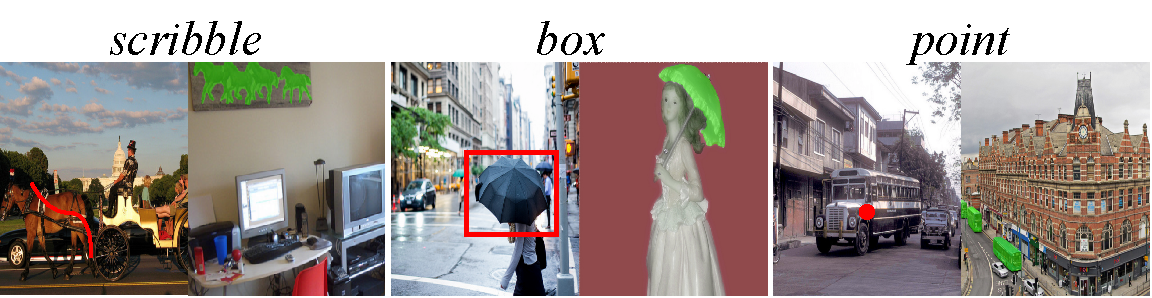
\includegraphics[width=\textwidth]{images/promptable.pdf}
    \caption{\textbf{Promptable few-shot segmentation with \ours{}.} Top: performance in strict few-shot (COCO-20$^i$) using different prompt types compared with VRP-SAM. Bottom: qualitative examples with point, scribble, and box prompts.}
    \label{fig:promptable_combined}
\end{minipage}

\end{figure*}
